% \subsection{Results}


\begin{figure}[tb]
    \begin{minipage}[h]{0.27\linewidth}
    \center{
        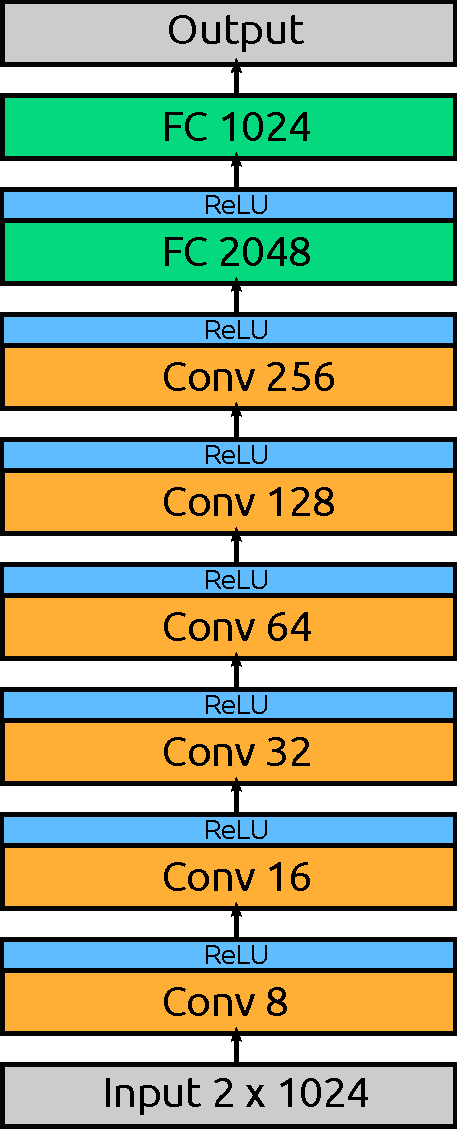
\includegraphics[width=1\linewidth]{images/nn_nft_inft/architecture_1.pdf} (a)
    }
    \end{minipage}
    \hfill
    \begin{minipage}[h]{0.72\linewidth}
        \begin{minipage}[h]{1.0\linewidth}
        \center{
            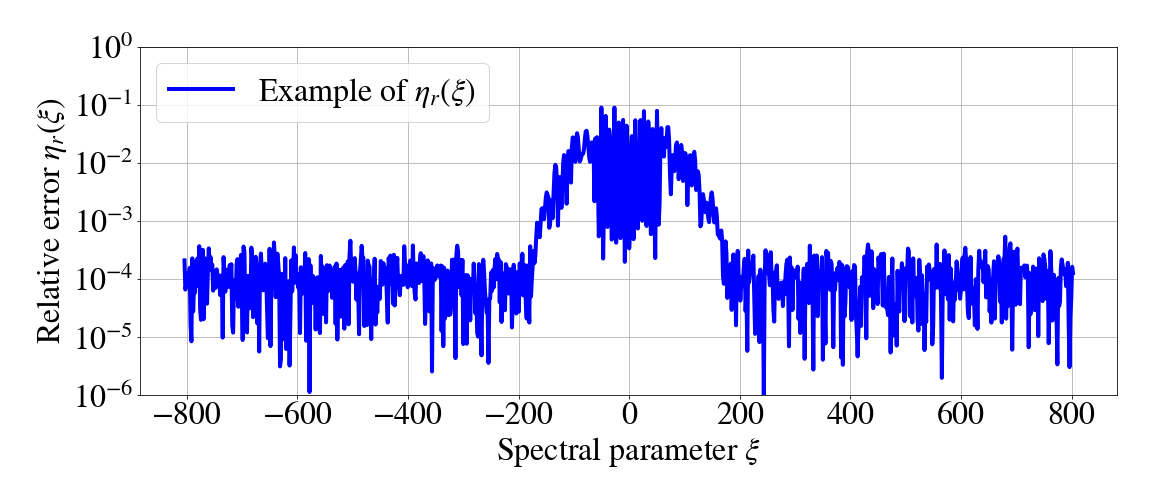
\includegraphics[width=1\linewidth]{images/nn_nft_inft/spectrum_rel_error_example_globecom.png} (b) \\
        }
        \end{minipage}
        \vfill
        \begin{minipage}[h]{1.0\linewidth}
        \center{
            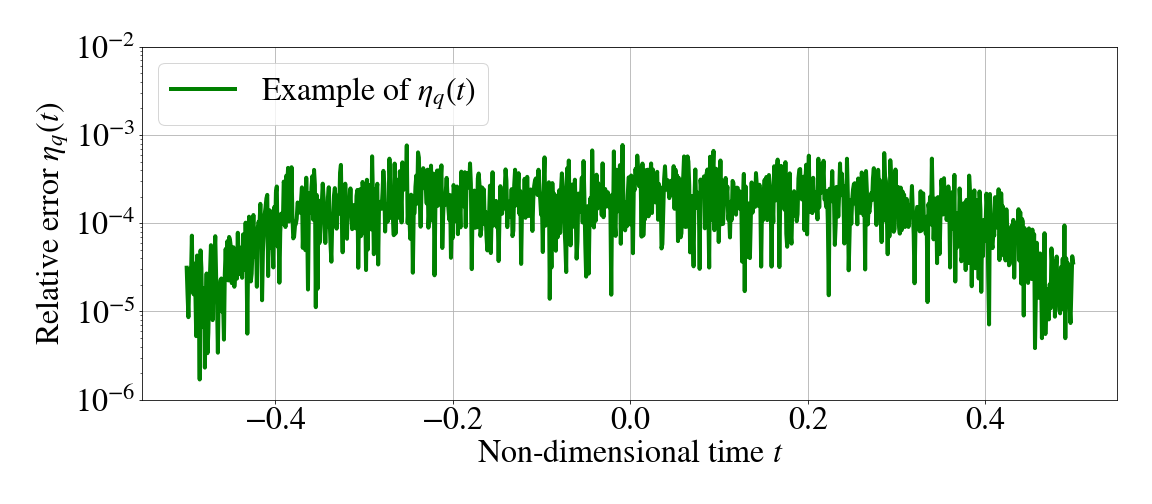
\includegraphics[width=1\linewidth]{images/nn_nft_inft/signal_rel_error_example_globecom.png} (c)
        }
        \end{minipage}
    \end{minipage}
    \caption{\textbf{(a)} Proposed architecture of the \acrshort{nn} that performs the NFT operations. \textbf{(b)} Value of the relative error $\eta_r(\xi)$ between the precomputed and predicted continuous spectrum. \textbf{(c)} Value of the relative error $\eta_q(t)$ between the original and predicted signal.}
    \label{fig:arch_and_result_nn_nft}
\end{figure}

In this section, we use the \acrshort{nn} to predict the continuous \acrshort{nft} spectrum of complex optical signals and transform the spectrum back (the inverse \acrshort{nft}) into a signal. 
\acrfull{cnn} are preferred over \acrfull{fnn} due to their efficient processing of spatial hierarchies in data. This efficiency makes \acrshort{cnn}s particularly suitable for tasks where context and locality play critical roles. Unlike \acrshort{fnn}s, which rely on simple matrix multiplications that cannot capture complex spatial relationships, \acrshort{cnn}s utilize layers equipped with convolutional filters. These filters are adept at capturing spatial features at various levels of abstraction, thereby allowing \acrshort{cnn}s to identify patterns more effectively. The significance of this capability becomes especially apparent in the context of the Nonlinear Fourier Transform. \acrshort{nft}, not being a linear transformation, means the local context within a time sequence greatly influences the outcome of the transformation. This nuanced influence of local context is something \acrshort{cnn}s can handle well, thanks to their spatial processing capability. For the random number generator, both here and in subsequent sections, I employ the Mersenne Twister as the core algorithm. This choice is due 
to its well-documented high-quality randomness and its exceptionally 
long period ($2^{19937}-1$), as detailed by Matsumoto and Nishimura (1998)~\cite{matsumoto1998mersenne}.

To assess the quality of the \acrshort{nn} prediction, we use the following formula defining the relative error for the continuous \acrshort{nft} spectrum:
\begin{equation}
    \eta_r(\xi) = \frac{|r_\text{predicted}(\xi) - r_\text{actual}(\xi)| }{\langle |r_\text{actual}(\xi)| \rangle_{\xi}} {,}
\end{equation}
where $\langle \cdot \rangle_{\xi}$ denotes the mean over the spectral interval, the ``predicted'' and ``actual'' indices refer to the \acrshort{nn}-predicted and precomputed values of the reflection coefficient $r(\xi)$, respectively. A similar formula for calculating the relative error for signal prediction:
\begin{equation}
    \eta_q(t) = \frac{|q_\text{predicted}(t) - q_\text{actual}(t)| }{\langle |q_\text{actual}(t)| \rangle_{t}} {,}
\end{equation}
where $q(t)$ is a signal and $\langle \cdot \rangle_{t}$ here is the mean over the time interval. The above relative error $\eta_r(\xi)$ and $\eta_q(t)$ is determined at the point $\xi$ and $t$, respectively. We use $\langle \eta_r(\xi) \rangle_{\xi}$ and $\langle \eta_q(t) \rangle_{t}$ to estimate the overall mean of the error. We stress that the metric was chosen in such a way as to take into account even the regions where the value of the spectrum or signal is much less than one.

% \begin{figure}[tbp]
% \centerline{
%     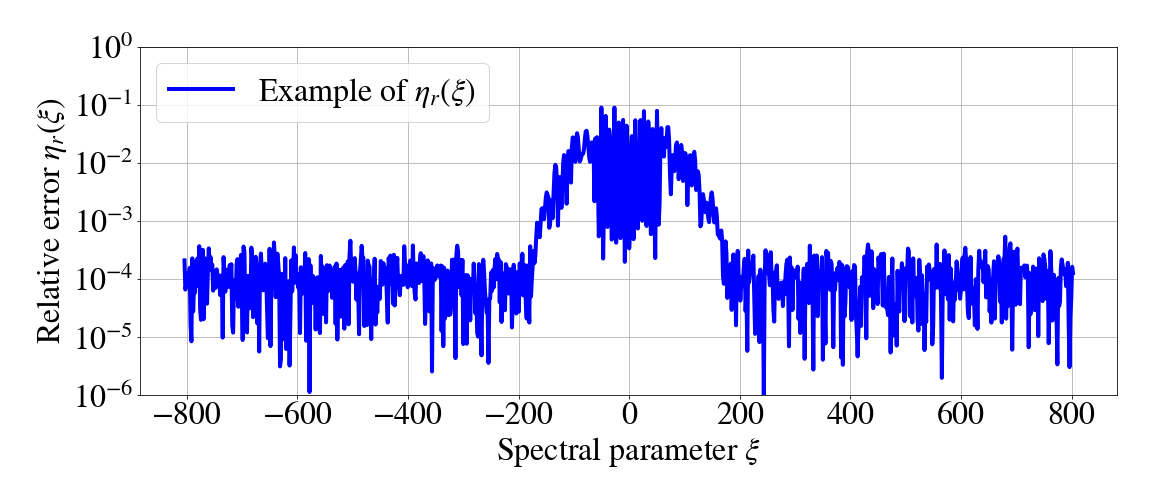
\includegraphics[width=1\linewidth]{images/nn_nft_inft/spectrum_rel_error_example_globecom.png}
% }
% \caption{Value of the relative error $\eta_r(\xi)$ between the precomputed and predicted continuous spectrum.}
% \label{fig:result_direct}
% \end{figure}

% \begin{figure}[tbp]
% \centerline{
%     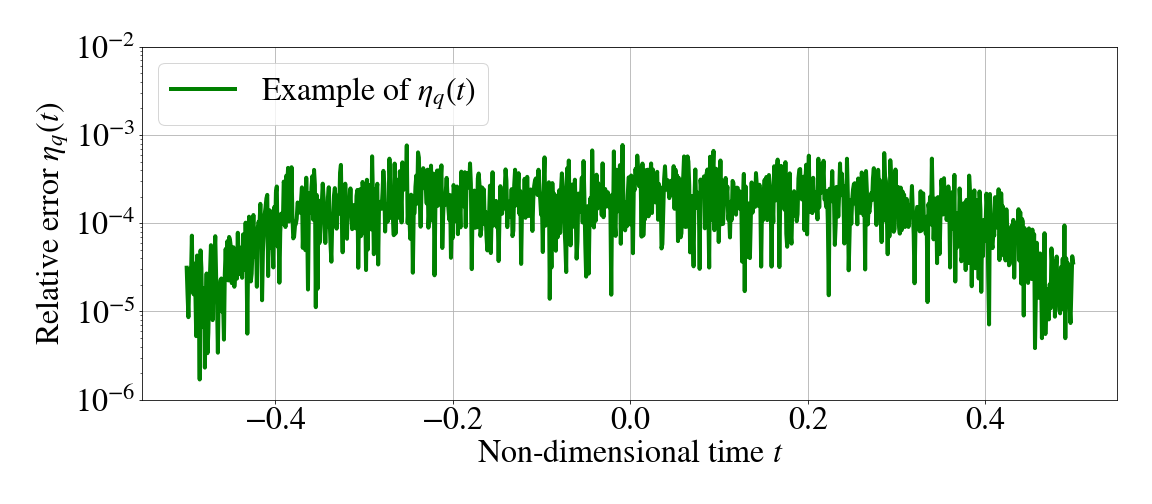
\includegraphics[width=1\linewidth]{images/nn_nft_inft/signal_rel_error_example_globecom.png}
% }
% \caption{Value of the relative error $\eta_q(t)$ between the original and predicted signal.}
% \label{fig:result_inverse}
% \end{figure}




Fig.~\ref{fig:arch_and_result_nn_nft}a shows the architecture of the \acrshort{nn} that performs the \acrshort{nft} operations (direct and inverse transform), with the parameters given inside the figure. The \acrshort{nn} consists of sequential convolution layers and fully connected output layers. At the input, the network receives a complex signal consisting of 1024 points. This \acrshort{nn} predicts only one component of the continuous NF spectrum, such that two identical \acrshort{nn}s have to be used to predict the real and imaginary $r(\xi)$ parts. Similarly, converting the spectrum back to a signal requires two separate \acrshort{nn}s for the real and imaginary parts of the signal $q(t)$. Each of the four \acrshort{nn}s with the same architectures we trained independently.

A total of 1024 points were selected to strike a balance between the computational complexity of the \acrlong{nft} and the demonstration of the \acrshort{nn} capabilities. This selection represents a synthetic case designed to start from simple signals, albeit with high resolution, to showcase the potential of \acrshort{nn}s to perform \acrshort{nft} operations. The choice of this specific number was motivated by its sufficiency to illustrate \acrshort{nn}s' ability to execute both forward and inverse \acrshort{nft}, while preventing the \acrshort{nn} model from becoming overly complex. Furthermore, the generation of the dataset required preliminary computations (i.e., performing \acrshort{nft}), and larger signal sizes would have necessitated more extensive calculation time.

There are 94035 signals in the dataset, 9403 are used for validation and are not involved in the training process. To generate the signals, we used random data sequences encoded in the \acrfull{qpsk} format. The energy of all signals is the same and is chosen at such a level that nonlinear effects are strong. At the selected energy, some of the signals contained a discrete spectrum, but such signals did not get into the training dataset. The continuous spectrum for each signal had been precomputed using the conventional direct \acrshort{nft} methods. To train the \acrshort{nn}, we used the mean squared error (MSE) as the loss function. In training the \acrshort{nn}, we employed the Adam (Adaptive Moment Estimation) optimisation algorithm with a learning rate of 1e-4. On average, with the amount of data used, our learning process took 50 000 epochs. To detect and mitigate overfitting during the training process, we monitor the loss function value on a validation dataset, which is distinct from the training dataset to ensure it does not influence the training directly. Additionally, we employ an early stopping callback mechanism. This mechanism tracks the loss values for both the training and validation datasets. Should the validation loss begin to increase -- a phenomenon observed over a range of epochs, in our case, from 100 to 500 across different studies -- the training process is halted. This strategy allows us to save the model at its peak performance, effectively before the onset of overfitting.

Fig.~\ref{fig:arch_and_result_nn_nft}b depicts $\eta_r(\xi)$ -- the difference between the predicted and actual (precomputed using conventional \acrshort{nft} method) continuous nonlinear spectrum for the example signal, while Fig.~\ref{fig:arch_and_result_nn_nft}c shows the example of $\eta_q(t)$ for the inverse \acrshort{nft}. We see from the graphs that \acrshort{nn} performs both forward and inverse transformations with high accuracy. Some increase in the error at the centre for a continuous spectrum is associated with its localization in the middle. While at the edges of the spectral interval, $r(\xi)$ values tend to $0$. There is no such feature for the signal since it is evenly located over the entire time interval.
The mean value over the entire validation set of the mean relative prediction error of the continuous spectrum $\langle \eta_r(\xi) \rangle_{\xi}$ for \acrshort{nn} forward \acrshort{nft} is $2.68 \cdot 10^{-3}$. For the inverse transformation, the mean over the entire validation set of the mean relative signal prediction error $\langle \eta_q(t) \rangle_{t} = 1.62 \cdot 10^{-4}$.
The results obtained show that the presented architecture can perform forward and backward \acrshort{nft} with high accuracy.


%-------------------------------------------------- Conclusions Section ———————————————————————————%

% \subsection{Conclusions}

% At the moment, ML and NN are state-of-the-art technologies that are actively researched in the fields of nonlinear signal processing and optical communications.
% The proposed NN architecture demonstrates the fundamental possibility of using the NNs to analyze and (de)modulate the complex optical signals used in communications. This opens up the prospects for improving existing systems without the need for a deep understanding of the internal nonlinear processes that affect the quality of signal transmission.
% We would like to stress that the method proposed in our current work is only the first step in the development of methods for machine processing of optical signals. It can be used to create smart receivers with digital back-propagation algorithms based on NFT and NN.
% Our findings demonstrate that the use of NN can allow studying not only the internal structure but also generating new signals using autoencoders. The fundamental possibility of using NN for NFT, in fact, can set up new areas for research related to the analysis of inherently nonlinear signal's structure and evolution characteristics. The next step in this direction can be the generalization of the results obtained in our work for the sake of our addressing the case of symbol sequences and simulating signal propagation in the NLSE-type channels.